\chapter{Methodology}
\label{methodology}

\section{Project management methodology}
I will use a Feature Driven Agile method. Meaning the workflow will by cyclical and focus on iterating over designs and prototypes. This will involve:
\begin{itemize}
  \item Requirements elicitation.
  \begin{itemize}
    \item This involves determening the needs of the user and defining requirements to meet those ends.
  \end{itemize}
  \item Feature design (UI).
  \begin{itemize}
    \item Features will be designed at first using wireframe models. Then on later iterations, colour and shading will be added alongside further usability considerations such as highlight on hover etc.
  \end{itemize}
  \item Feature implementation research.
  \begin{itemize}
    \item This step involves determining the apropriate technologies and libraries to achieve the design. This is nececarry to realize the constraints that are imposed by the implementation method and know to what extent the design is feasible.
  \end{itemize}
  \item Feature implementation.
  \begin{itemize}
    \item Writing the code to create the feature.
  \end{itemize}
  \item Feature testing.
  \begin{itemize}
    \item Initially testing will be done manually with valid values until later iterations whereby extraneous values will be introduced. Once the feature is in it's final iterations a unit test will be introduced.
  \end{itemize}
  \item Evaluation.
  \begin{itemize}
    \item Does the feature meet the requirements and fulfill the needs of the user?
  \end{itemize}
\end{itemize}
This workflow will consist of a single cyclical workflow, with two nested "sub workflows" whereby upon completion of a step, it is sometimes nececarry to loop back on oneself to perform futher refinement. As illustrated by the diagram below.
\begin{figure}
  \begin{center}
    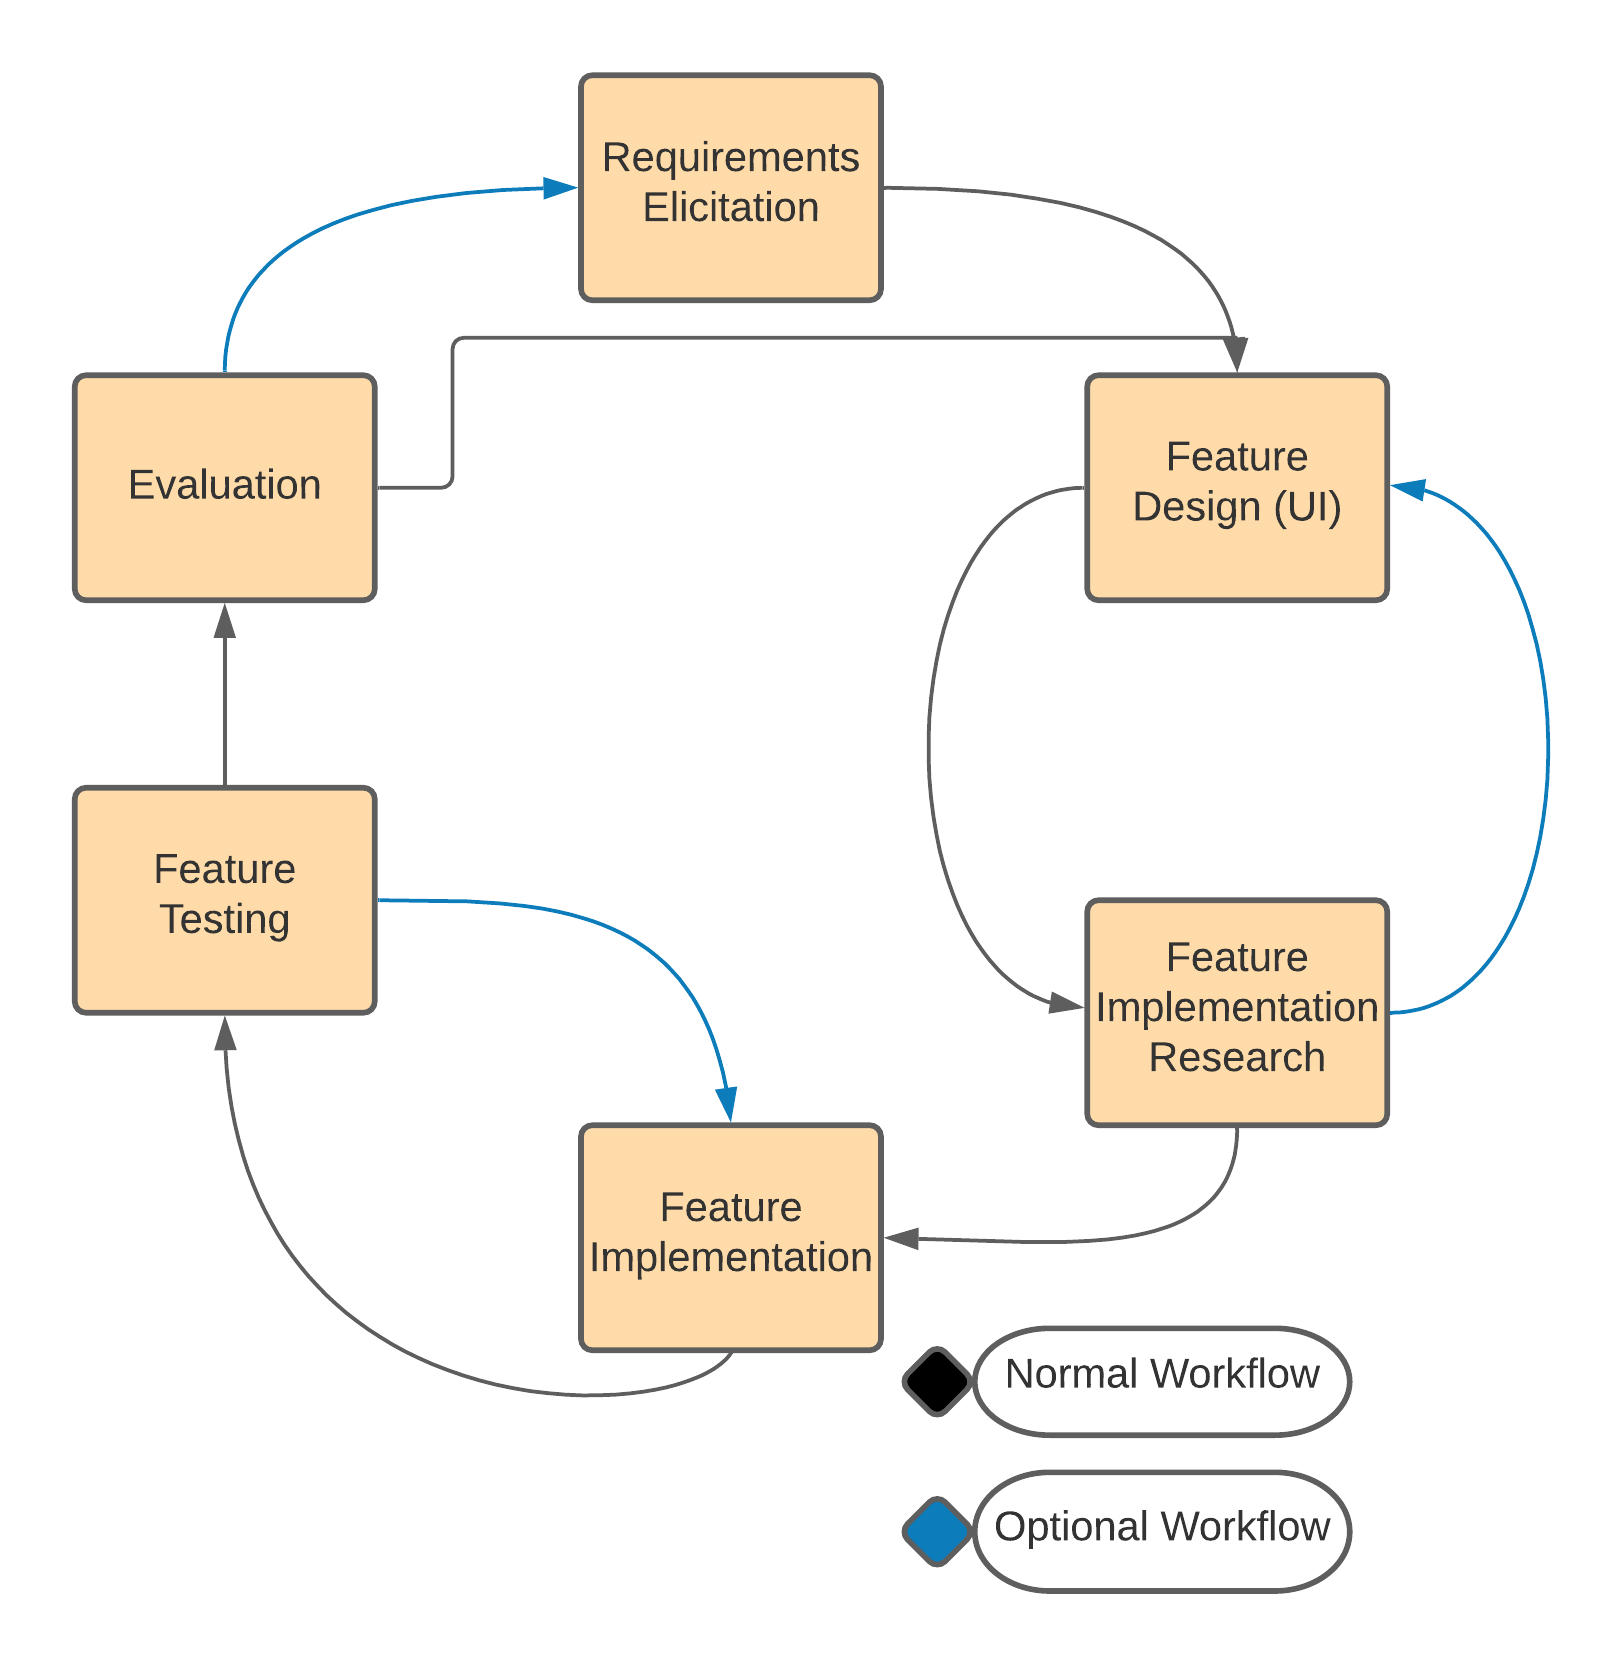
\includegraphics[scale=0.75]{Images/Project_Management_Methodology}
    \caption{Development Lifecycle}
    \label{fig:development lifecycle}
  \end{center}
\end{figure}
Throughout the project the focus of the workflow will shift as illustrated by the diagram below.

\begin{figure}
  \begin{center}
    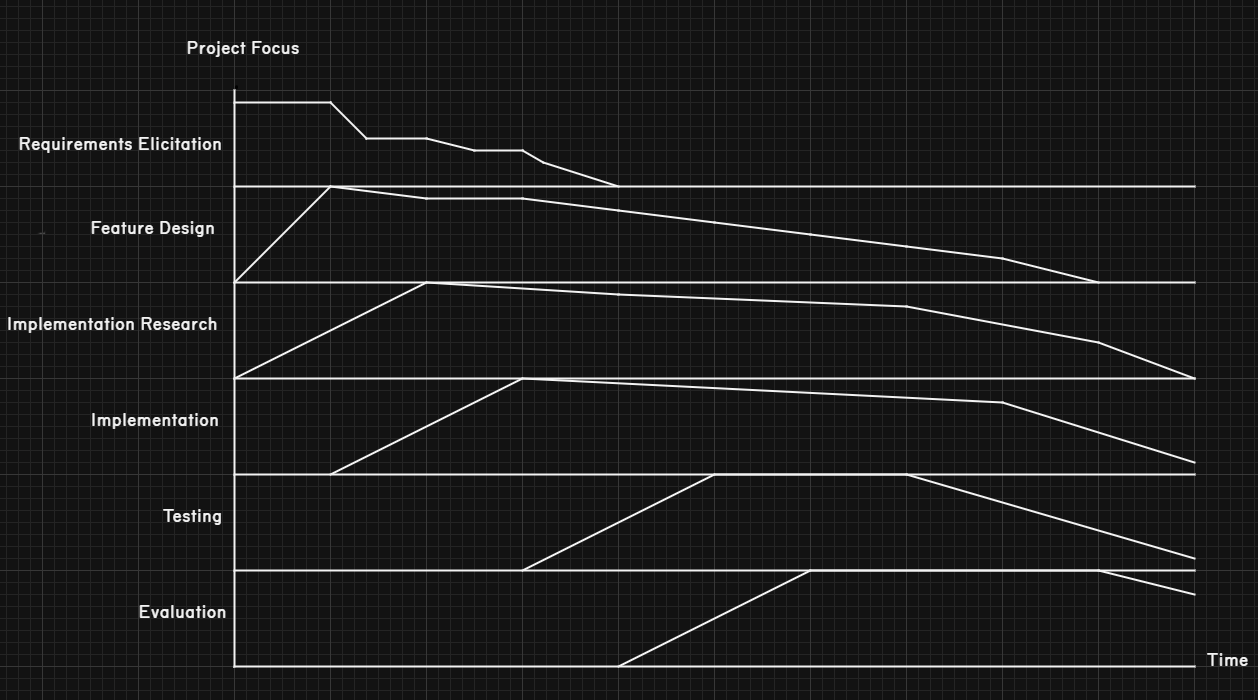
\includegraphics[scale=0.4]{Images/ProjectFocus2}
    \caption{Project Focus Over Time}
    \label{fig:project focus}
  \end{center}
\end{figure}

The paper [CITE BIS OF INNOV] makes a compelling argurment for the usage of agile methodologies over more linear project management methodology (PMM) styles such as waterfall. Agile focuses on design being done 'on an ongoing bases in smaller chunks' [CITE BIS OF INNOV]. It is also highlighted that agile allows development to respond to feedback and change. In fact agile has customer, designer and developer feedback baked in to it's formula in the form of regular team meetings, especially if using the SCRUM 'flavour'.
\par
For a lone developer Agile with Kanban is the PMM of choice as it allows the flexebility to iterate on designs as one learns more about the technologies being used and gives the freedom to modify one's requirments in light of newly found research and technical limitations. Aditionally the nature of agile is to haves short lifecycles which has the virtue of frequent milestones. This allows one to better track progress of the project by being able to see how many tasks have been completed on the Kanban board during the development cycle\footnote[4]{Granted tasks alone are not the be-all, end-all metric but it does give some idea of progress}.
\par
Using Kanban to track tasks makes sense for a single developer as appose to using feature driven development. As this allows for non-programming tasks to be tracked in the same way as programming tasks.
\par
Furthermore, agile is a worthwhile methodology to use and familiarise oneself with as it has become the new norm in industry. As shown by a study conducted by Hewlett Packard.

\begin{figure}[H]
  \begin{center}
    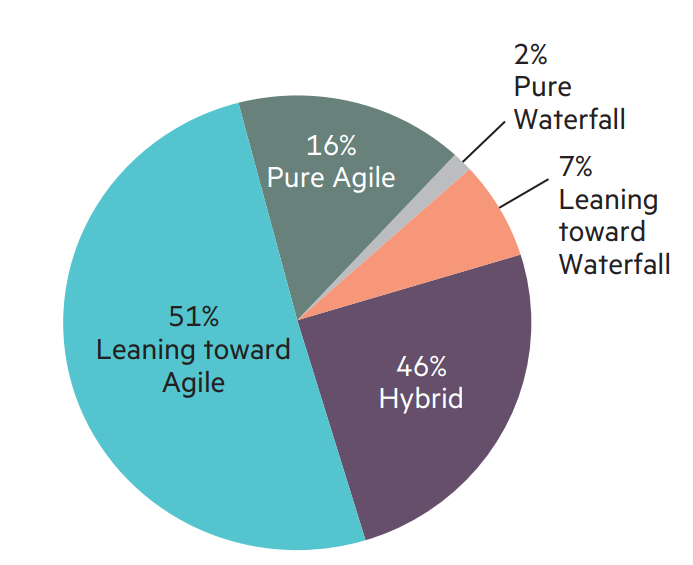
\includegraphics[scale=0.4]{Images/PMMPieChart}
    \caption{Primary development method used in organization across projects (601 respondents) diagram created by Hewlett Packard}
    \label{fig:PMM_PieChart}
  \end{center}
\end{figure}

While creating the product one's goal will be to implement a Minimum Viable Product (MVP). Defined by a product that fulfils the 'must have' requirements before expanding it's features to include 'could have' features etc. Aditionally, once the MVP is acheived, design considerations such as ease of extensability and addition of new features will be more heavily focused on. Sometimes with major code refactor occuring at this point, as to acheive the MVP quickly it is sometimes nececarry to 'hard code' parts or implement features in a way that may not be conducive to easy maintinence or serving content dynamically.

\section{Evaluation Design}
  This will be conducted by linking users to the website with a link to an online survey alongside a link to a google drive folder containing relevant test images. With the questionaire mostly consisting of System Usability Survey (SUS) questions. And some aditional bespoke questions regarding accuracy of prediction.
\section{Requirements Elicitation}
  As the scope of the problem domain is narrow in terms of interaction points for the user. Requirment elicitation will be driven by determining features that will build towards the solving the problem at hand. If for instance the problem was providing some kind of E-commerce website, project management application or social media website, the number of different features that could be employed in any one of these domains is vast and therefore one would need to consult the target audience and elicit the kind of requirements they would like to have. On the contrary, this project is far narrower in terms of points of interaction for the user. Therefore requirements will be determined on the basis of whether or not they contribute towards providing information about crop defects to the user.
  \par
  This is not to say user feedback is not useful for this project it still a good way to be alterted to any usability issues. Such as bugs, difficulty understanding how to use the application (what icons mean, order to carry out steps etc) and difficulty seeing UI elements due to poor colour choice. And for other projects with a specific customer in mind can use customer feedback to determine for instance how the program should handle erronus data. Or is it imperative that this program exececutes quickly? Or will the client be handling sensitive data and need to have the security of the application in mind?

\section{Feature management}
  To track the creation and completion of features, a Kanban board will be used. This will include columns for 'To do', 'Doing' and 'Done'.
  To determine which features will be prioritised one will employ the MOSCOW method see Feature Management.

\section{Design Methods}
   \begin{itemize}
     \item Requirements Elicitation
     \begin{itemize}
       \item To better conceptualize the needs of the user. Use case diagrams and activity diagrams will be utilized.
     \end{itemize}
     \item User Interface
     \begin{itemize}
       \item Wireframes will be uitilized to establish interface element placement i.e. layout.
       \item More detailed mockups will be created when the earlier wireframes are constructed as prototypes and the concept is proved acheivable.
       \item A colour picker will be utilized to define the colour scheme.
       \item In later iterations of the design, once there is a functioning UI,
       usability will continue to be refined with the help of existing usability research,
       to guide the usage of font/colour/highlight on hover/font size etc.
       \item Additionally once a desktop friendly layout has been established, work will begin on optimizing a version for mobile.
     \end{itemize}
     \item Back-End
     \begin{itemize}
       \item UML will be used to show the overall design of the system through structural diagrams. These will show the interfaces of the classes and how they will interact with one another.
     \end{itemize}
   \end{itemize}

\section{Testing methods}
  Testing will be conducted iterativley as the functionality expands, with unit tests being introduced for some components depending on time constraints. Testing will consist of firstly confirming that when interfaces are interogated with sound data, the responses are consistent with requirments. And secondly stress testing the interfaces with extraneous data to ensure that apropriate error responses are given and the application does not simply crash. And if in the case of crashing, is able to automatically re-start.

\section{Version control}
  I will be using Git and Github. This will allow the creation of branches to explore experimental parts of the soloution space without disrupting the progress of the main branch. If the experimental implementation is successfull it will be merged with the main branch. It also allows the development of features in paralel, with any conflicts in their implementation being resolved at the merge stage. The inclusion of a remote repository allows for work to continue on a seperate machine if nececarry and later be synced with the local main branch.
  \begin{figure}[H]
    \begin{center}
      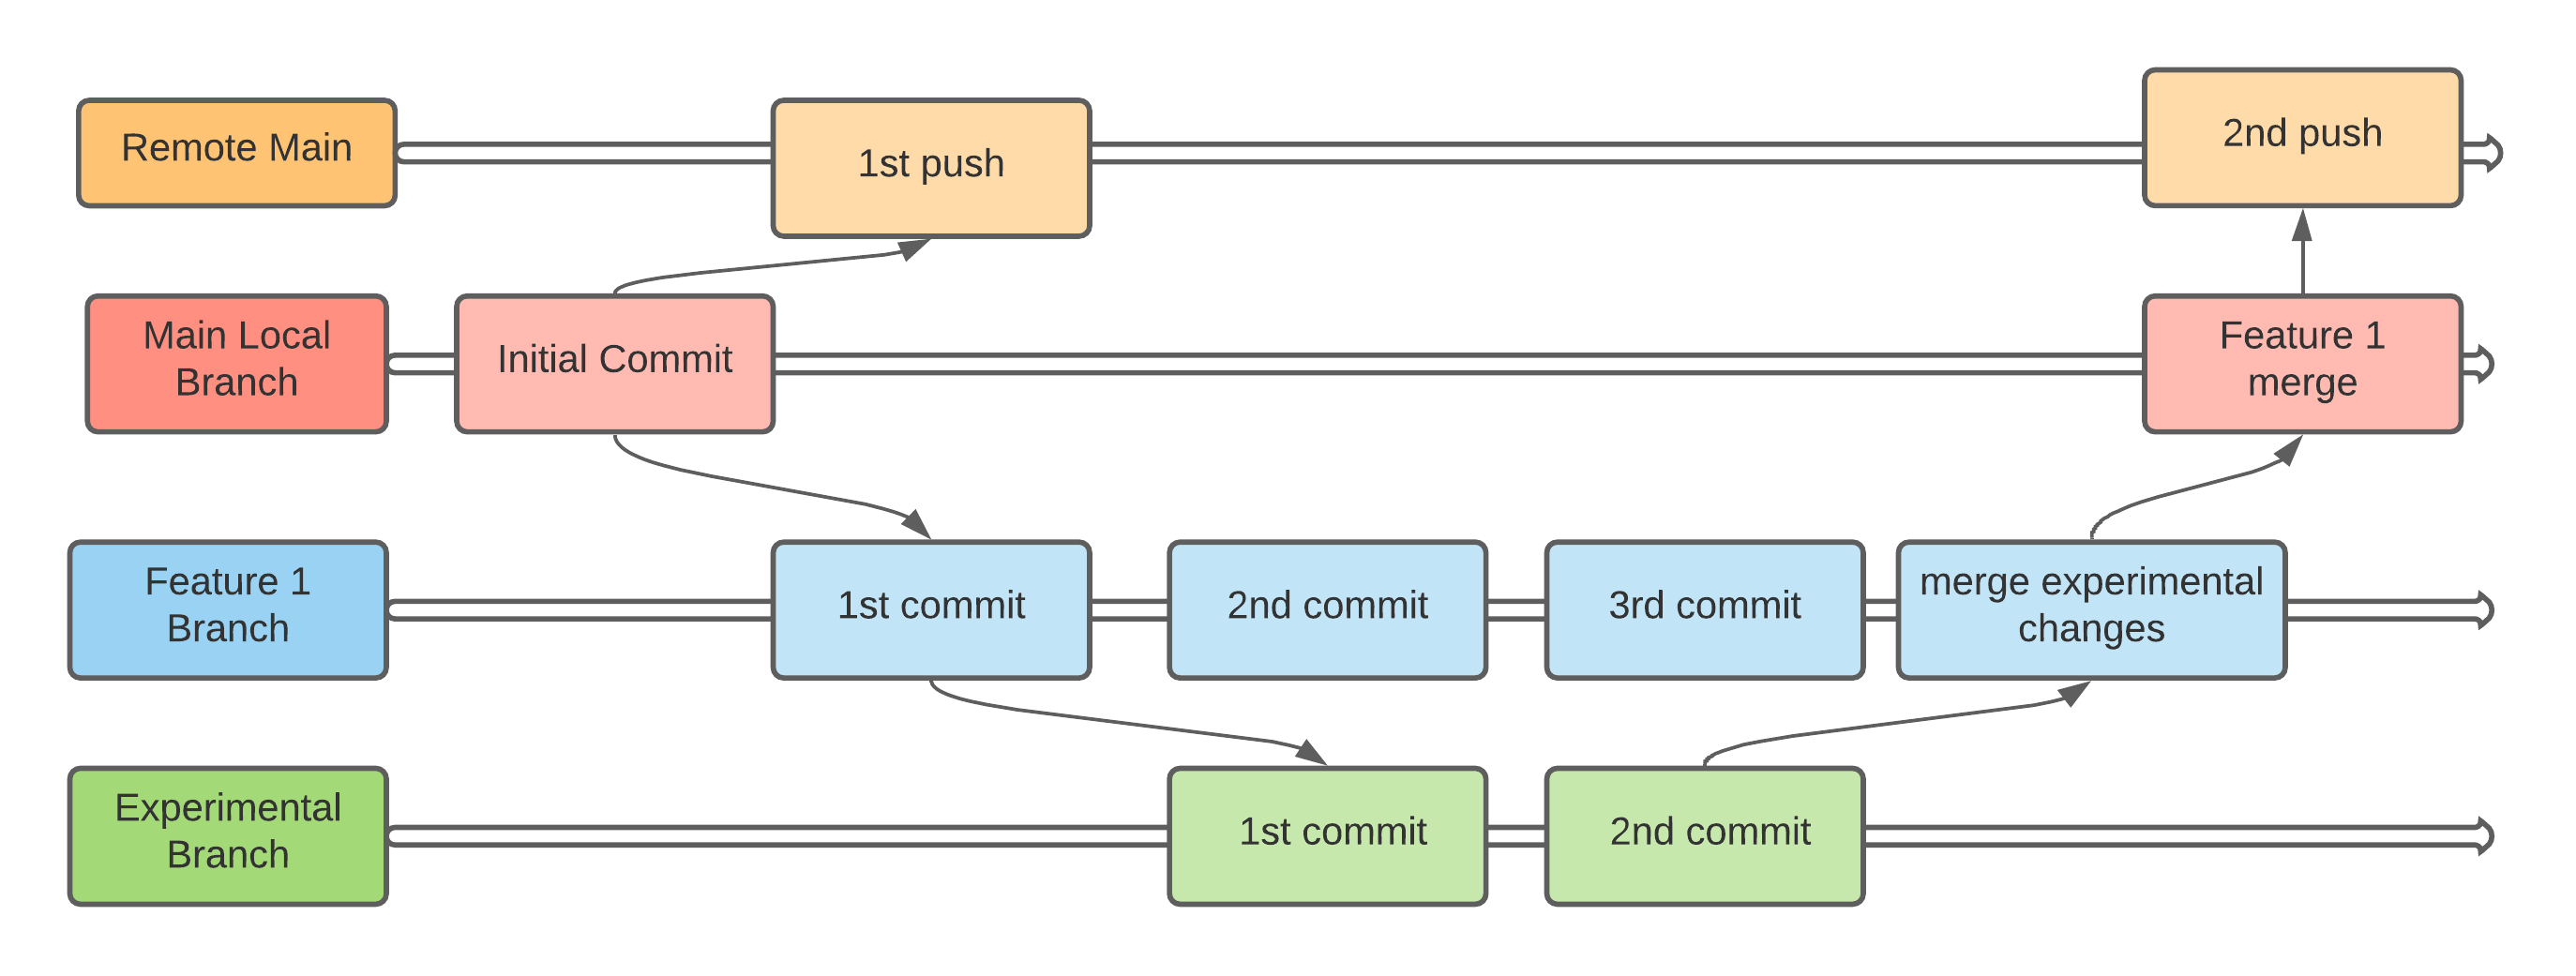
\includegraphics[scale=0.7]{Images/Git_Workflow_Diagram}
      \caption{Example Workflow To Highlight Branch Usage}
      \label{fig:Git Workflow}
    \end{center}
  \end{figure}

\section{Evaluation methods}
  \subsection{User Interface}
  The main method that will be utilized to determine the quality of the user interface will be the System Usability Scale (SUS) which can be seen here. (CITATION) % insert reference here
  The evaluator will be given remote access to the webservice. They will also be provided with some sample images to test the perfomance of the CNN incase they do not have suitable images of their own.
  The opinion data will be collected via online questionare.
  \subsection{Convolutional Neural Network (CNN)}
  Metrics for the evaluation of the CNN will be:
  \begin{itemize}
    \item Time to train the network on available hardware
    \begin{itemize}
      \item The constraint here being if the network cannot be trained on the available hardware in under sixteen hours. Purely for practical considerations.
    \end{itemize}
    \item Accuracy of CNN predictions. (which will be most effective when there are equal numbers of samples belonging to each class) $Accuracy = \frac{Correct Predicitons}{Total Predictions}$ Else if the samples are sqewed, the network could be a faliure at detecting a specific under-represented class, yet still score high accuracy.
    \item Precision. This is the number of correctly predicted images out of all predictions of that class. $Precision = \frac{Correctly Predicted for Class}{Total Predicted for Class}$ The network is precice for a class when the predictions it does make are correct. Precicion cannot be used in isolation due to the fact that the network can have a high precicion for a class but still fail to identify the majority of images for that class. Succeeding soley on the fact that the images it has classified are correct.
    \item Recall. Is the correct number of predictions for a class out of the number present of that class. $Recall = \frac{Correct Predicted for Class}{No. Present For Class}$
    This metric can also not be used in isolation due to the fact it does not take in to account the number of false positives. i.e. The number of images incorectly classified as the class in question. For example, if an image dataset contained three classes A, B, C, and the classfiier labeled all images A. The recall for A would be 100 percent.
    \item F1 score. This metric tries to find the balance between precision and recall and can be expressed as $F1 = 2 \times \frac{1}{\frac{1}{precicion} + \frac{1}{recall}}$
  \end{itemize}
\section{Initial Designs}
Firstly I have created a wireframe UI
  \begin{figure}[H]
    \begin{center}
      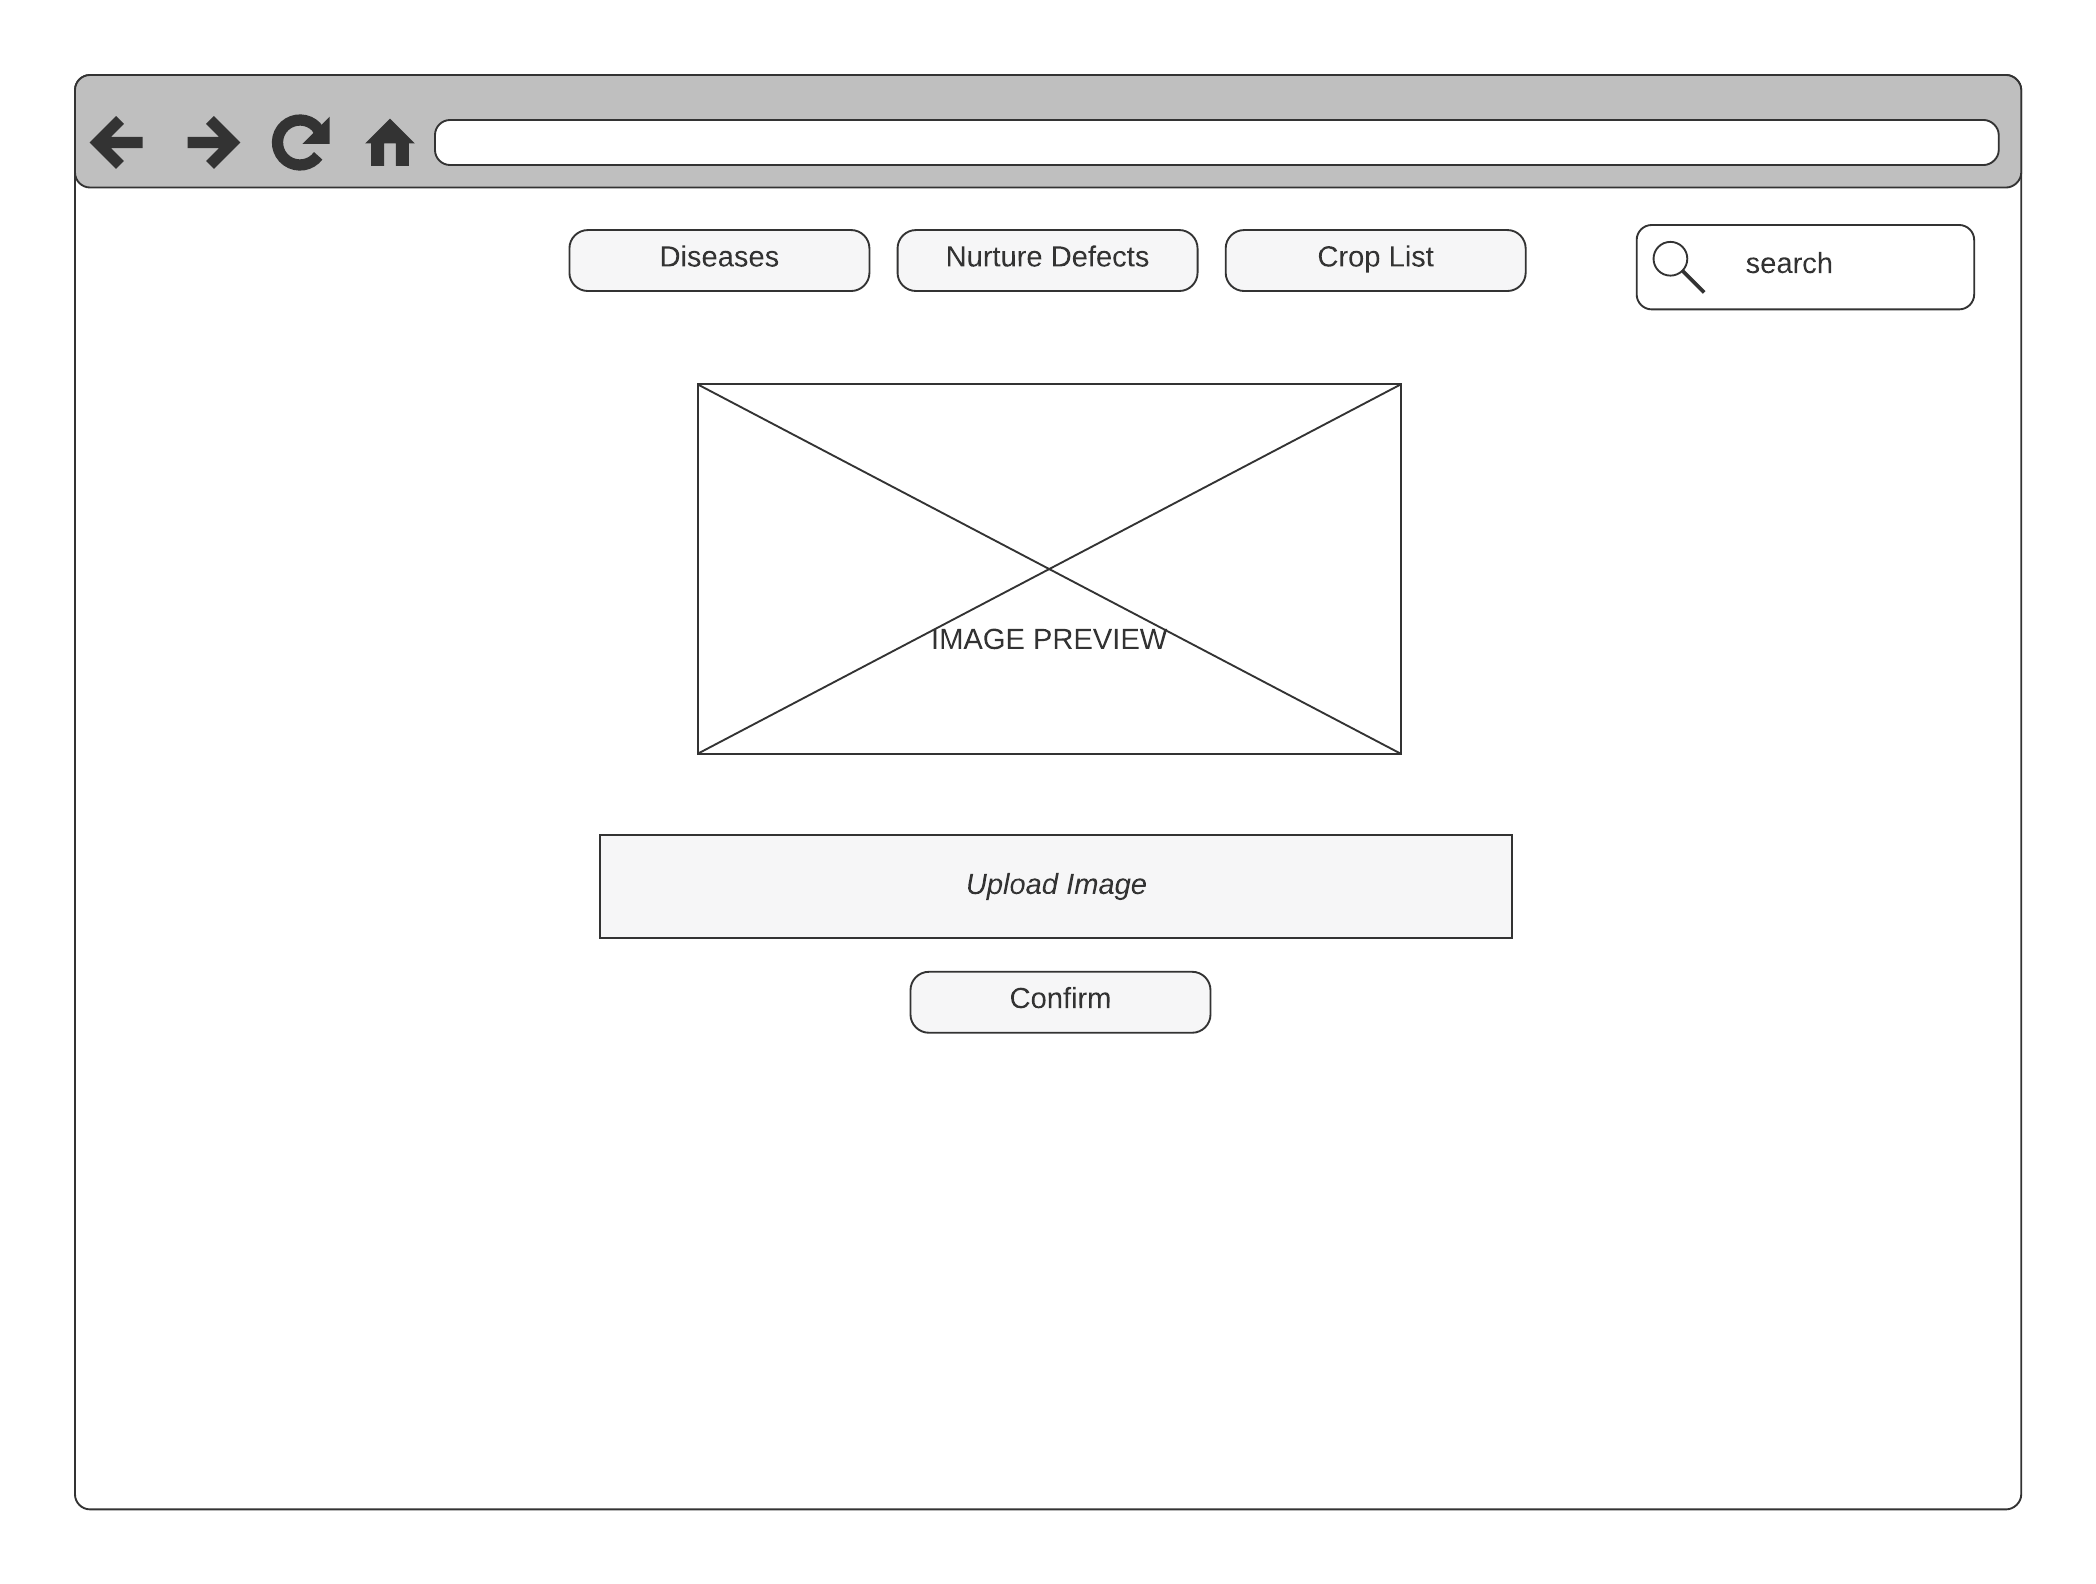
\includegraphics[scale=0.7]{Images/Home_Page_Wireframe}
      \caption{Homepage Wireframe}
      \label{fig:homepage_wireframe}
    \end{center}
  \end{figure}
  \begin{figure}[H]
    \begin{center}
      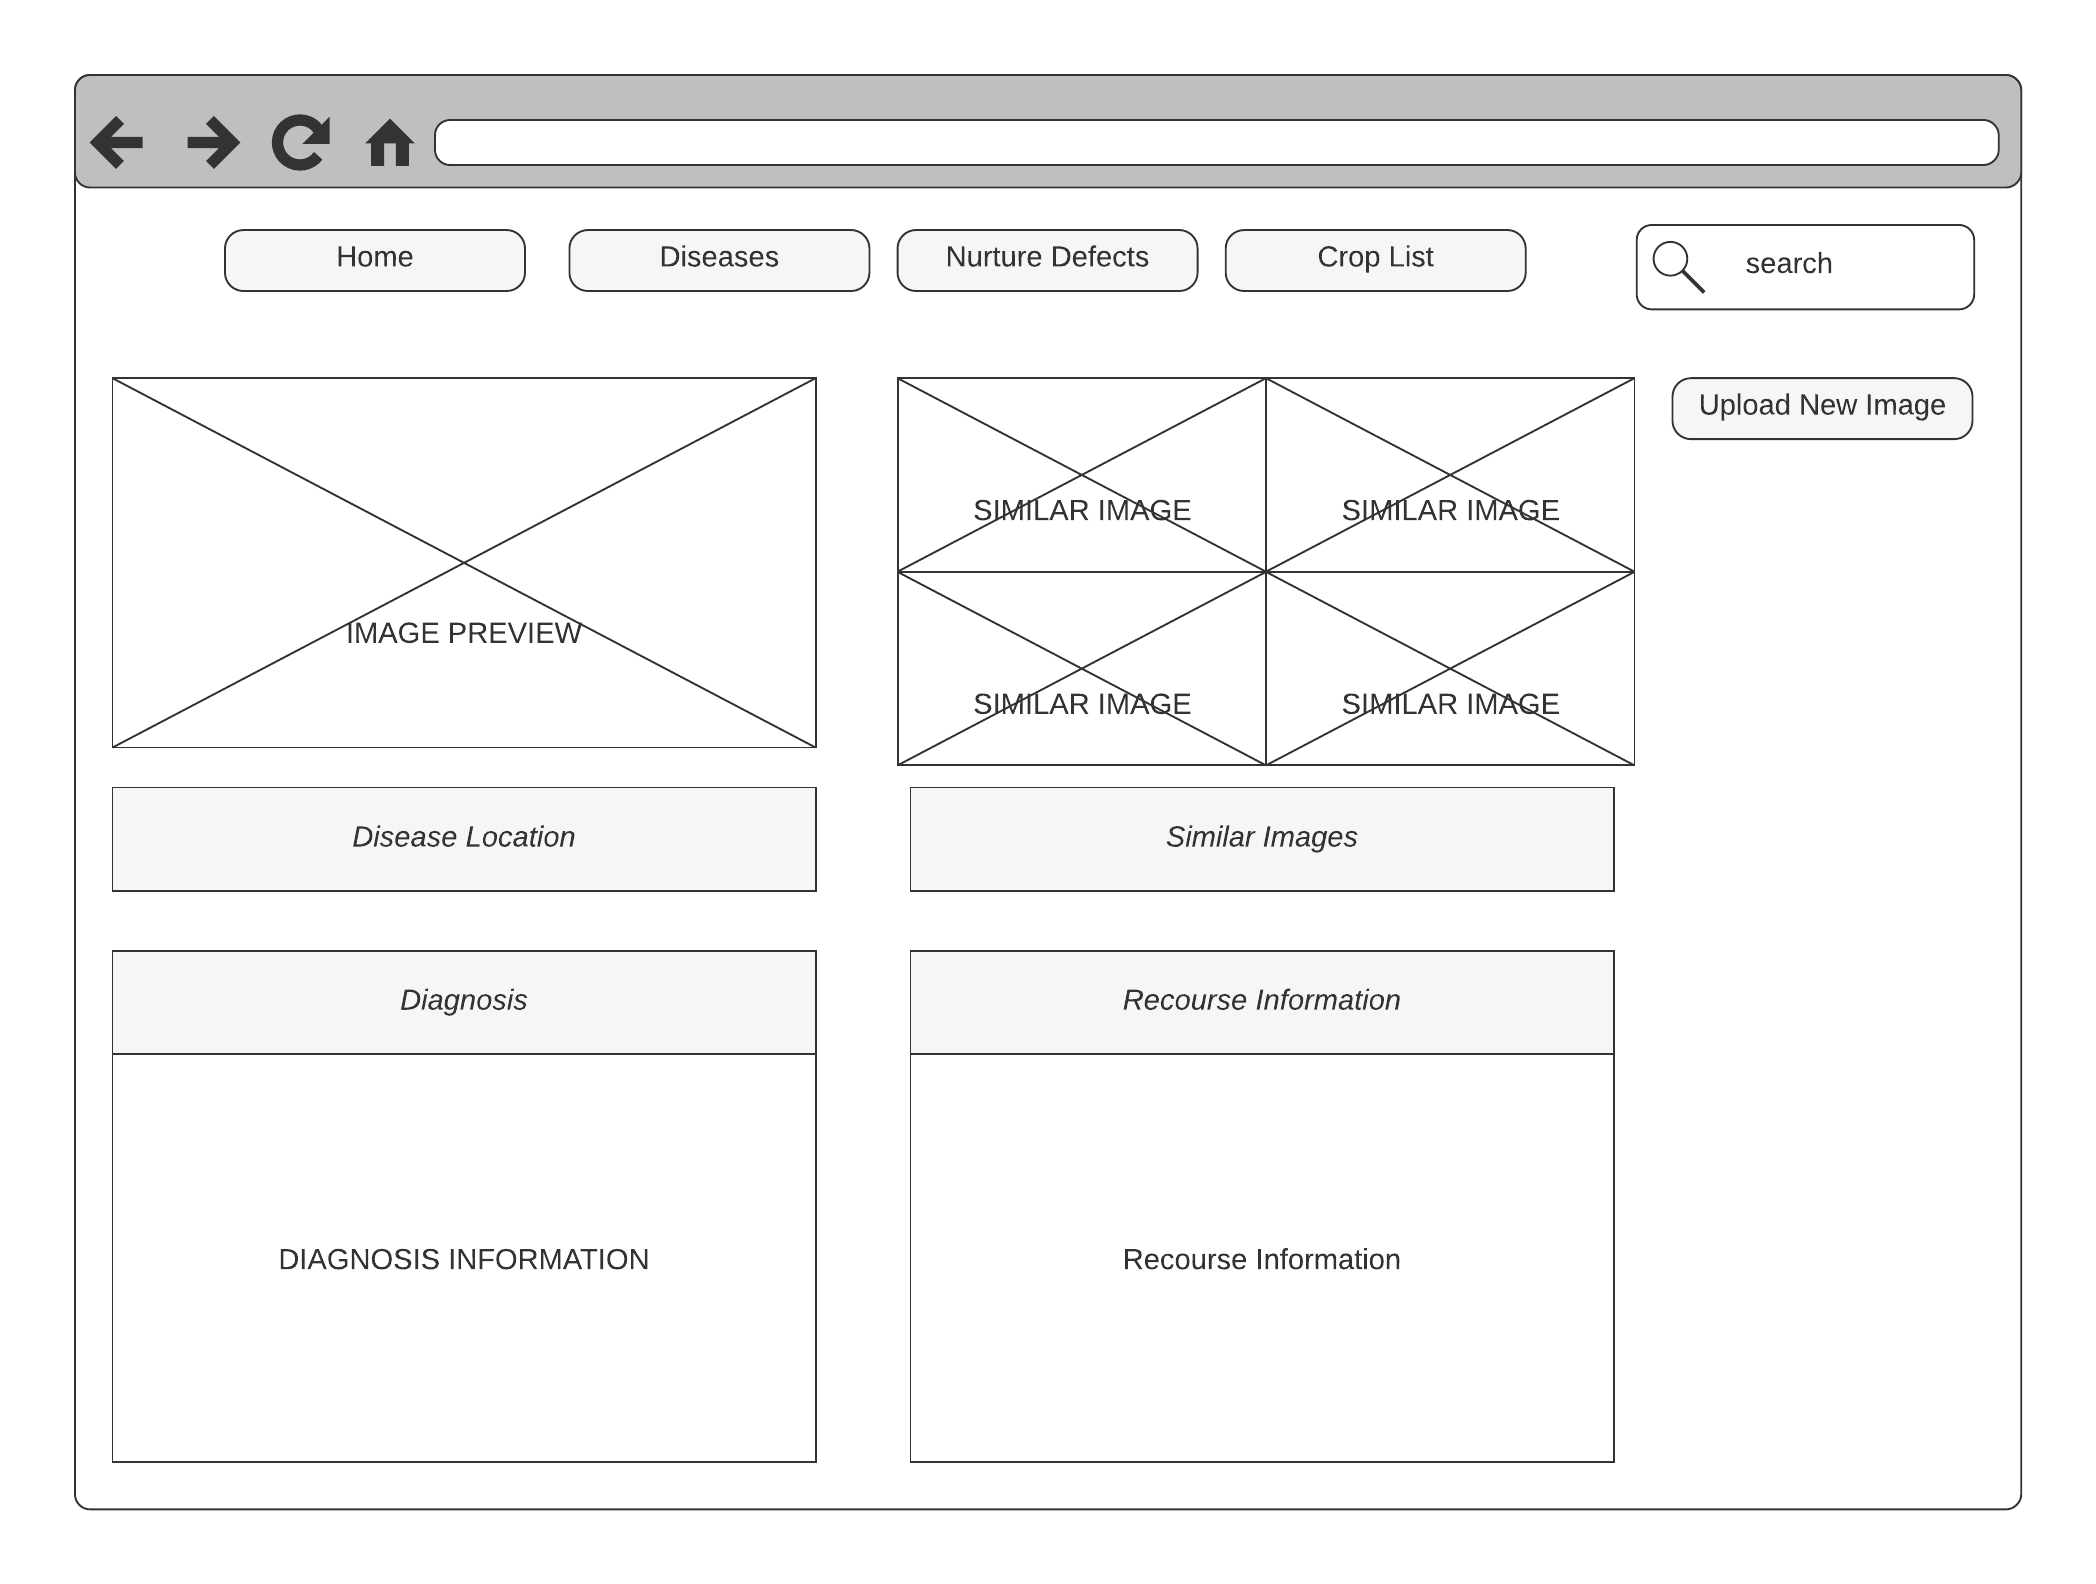
\includegraphics[scale=0.7]{Images/Defect_Information_Wireframe}
      \caption{Defect Information Wireframe}
      \label{fig:defect_wireframe}
    \end{center}
  \end{figure}
  \begin{figure}[H]
    \begin{center}
      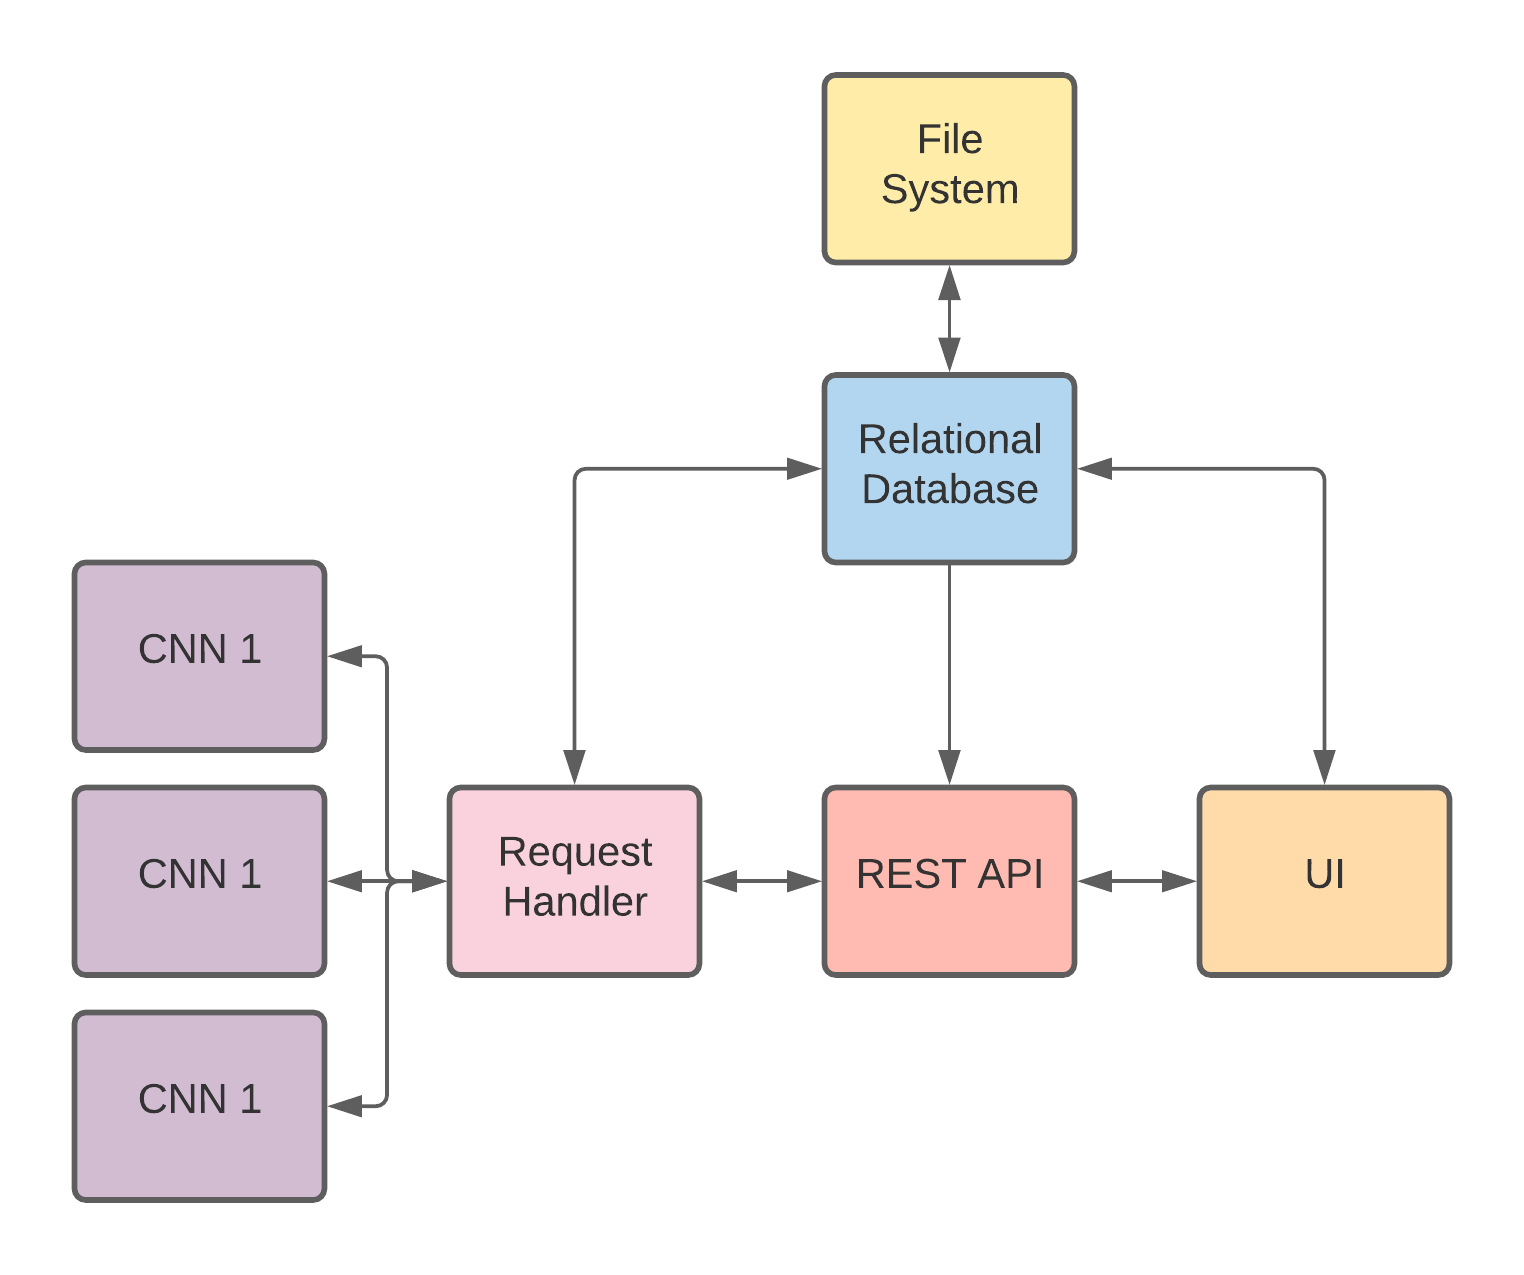
\includegraphics[scale=0.7]{Images/System_Overview_v1}
      \caption{System Overview}
      \label{fig:sys_overview}
    \end{center}
  \end{figure}
    \begin{figure}[H]
      \begin{center}
        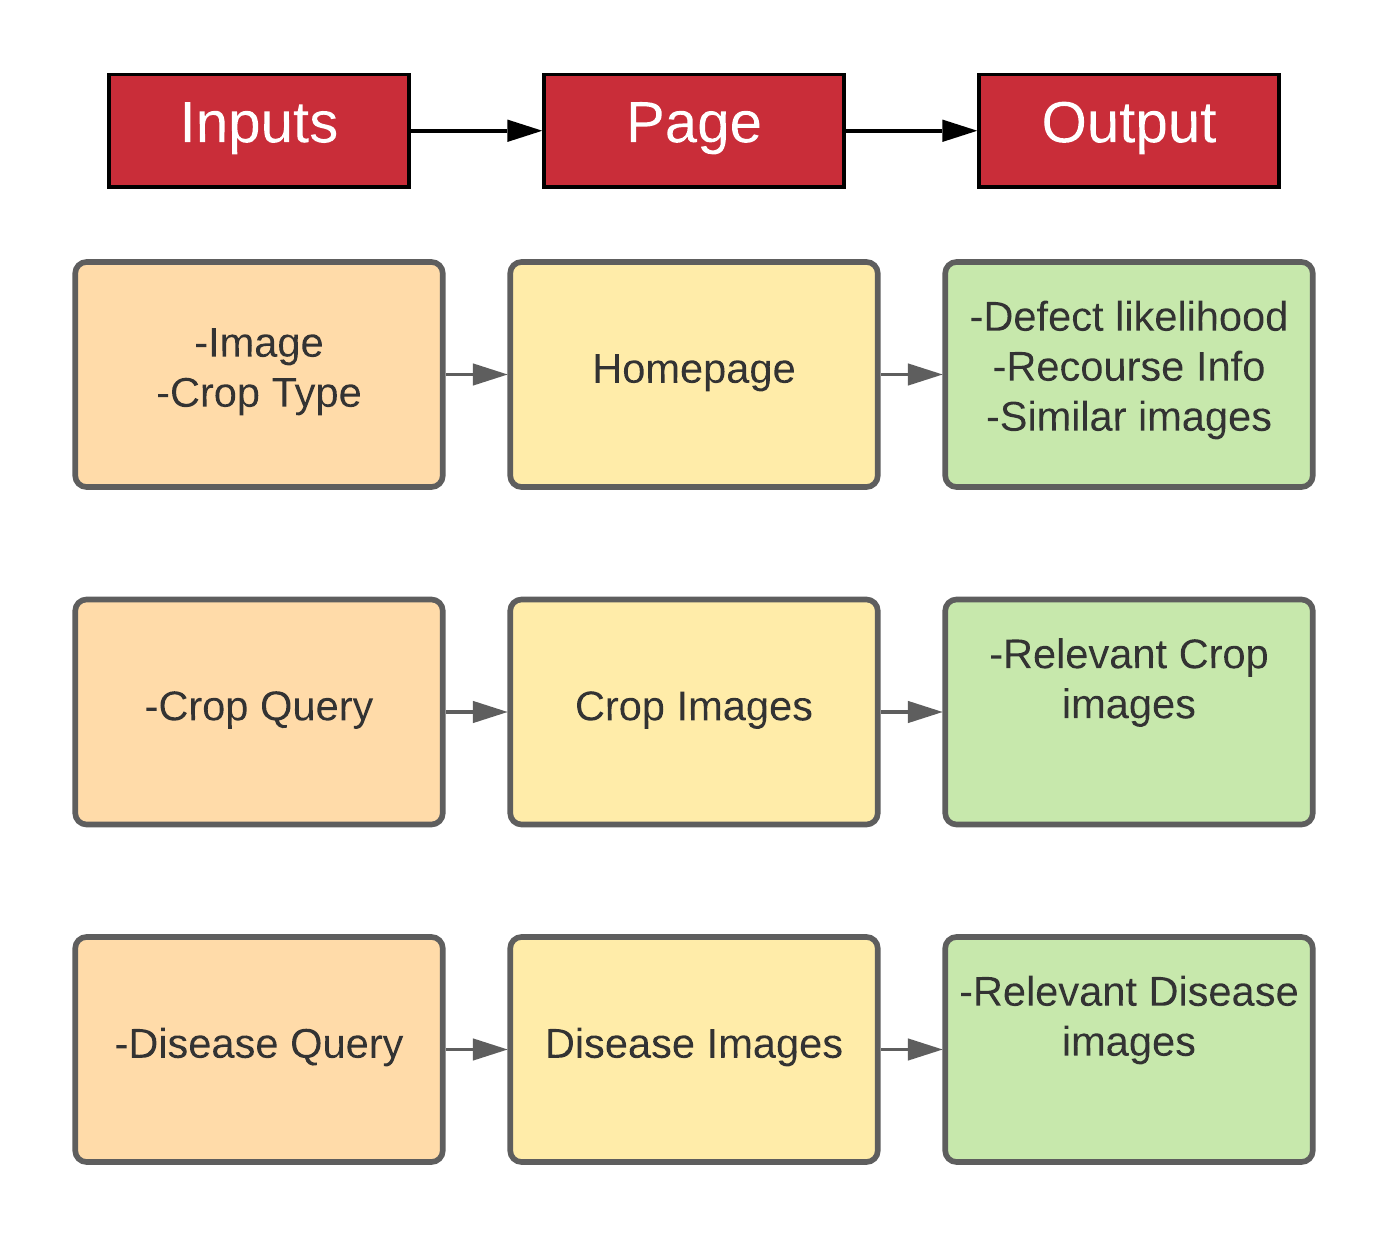
\includegraphics[scale=0.7]{Images/Input_Output_UI}
        \caption{Input/Output overview}
        \label{fig:input_output}
      \end{center}
    \end{figure}
    \begin{figure}[H]
      \begin{center}
        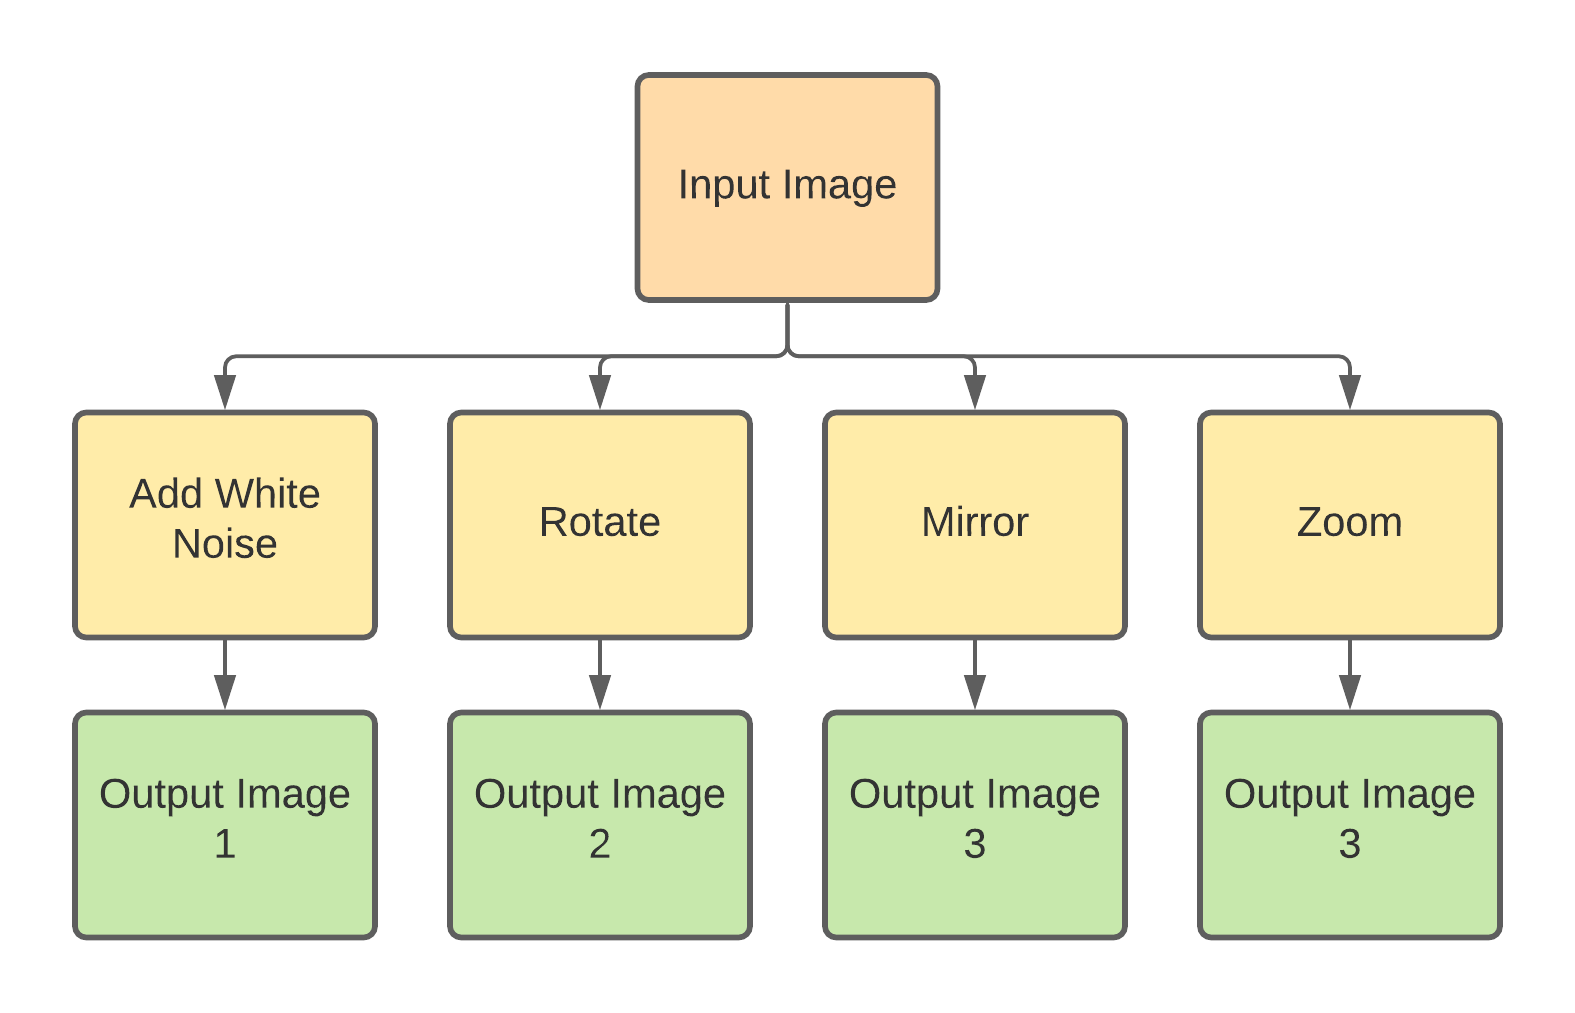
\includegraphics[scale=0.7]{Images/Data_Augmentation}
        \caption{Input/Data Augmentation Methods}
        \label{fig:data_augmentation}
      \end{center}
    \end{figure}
\section{Employed Technologies \& Justifications}
  \subsection{Software Structure}
    \subsection{Back-End}
      The design aims to seprate the functionality of the CNN and the User Interface (UI) through use of a Representational State Transfer (RESTFul) Aplication Interface (API). The central idea of this aproach is to allow a seperation of distinct components which allows for flexebility in managing updates and changes to each component. The 'backend' which in this context refers to the CNN and it's related functionality, such as processing it's input's and outputs; will both recieve input and serve it's output through the interface of the RESTFul API. each 'endpoint' or in other words internal class of the API will all inherit from the Resource interface which means it will get the main four HTTP protocol functions. POST, GET, PUT, DELETE. All interogations of the CNN will be conducted through these requests.
      \par
      A key feature of A RESTFul interface is the fact that no client information is stored
      between requests, this aids in making the interface more scalable and iteroperable. Scalable in the sense that increasing clients does not increase the amount of information the backend will have to store and interoperable in the sense that any client, be it mobile appliation, CLI program or webpage can use the interface.
      \par
      To increase orthogonality of the system, defect images are stored standalone on an image server. With the API serving the name of the defect which gives the information nececarry for the webpage to retrieve the correct images. This is because the directory structure of the image server is set up such that directory names are defect classes and all image names are numbers. Having the images stored on a seperate server rather than bundled with the front-end makes the service more useful. As it means any other interface can also choose to obtain the defect images (although image server endpoint information is not served by the API).

    \begin{figure}[H]
      \begin{center}
        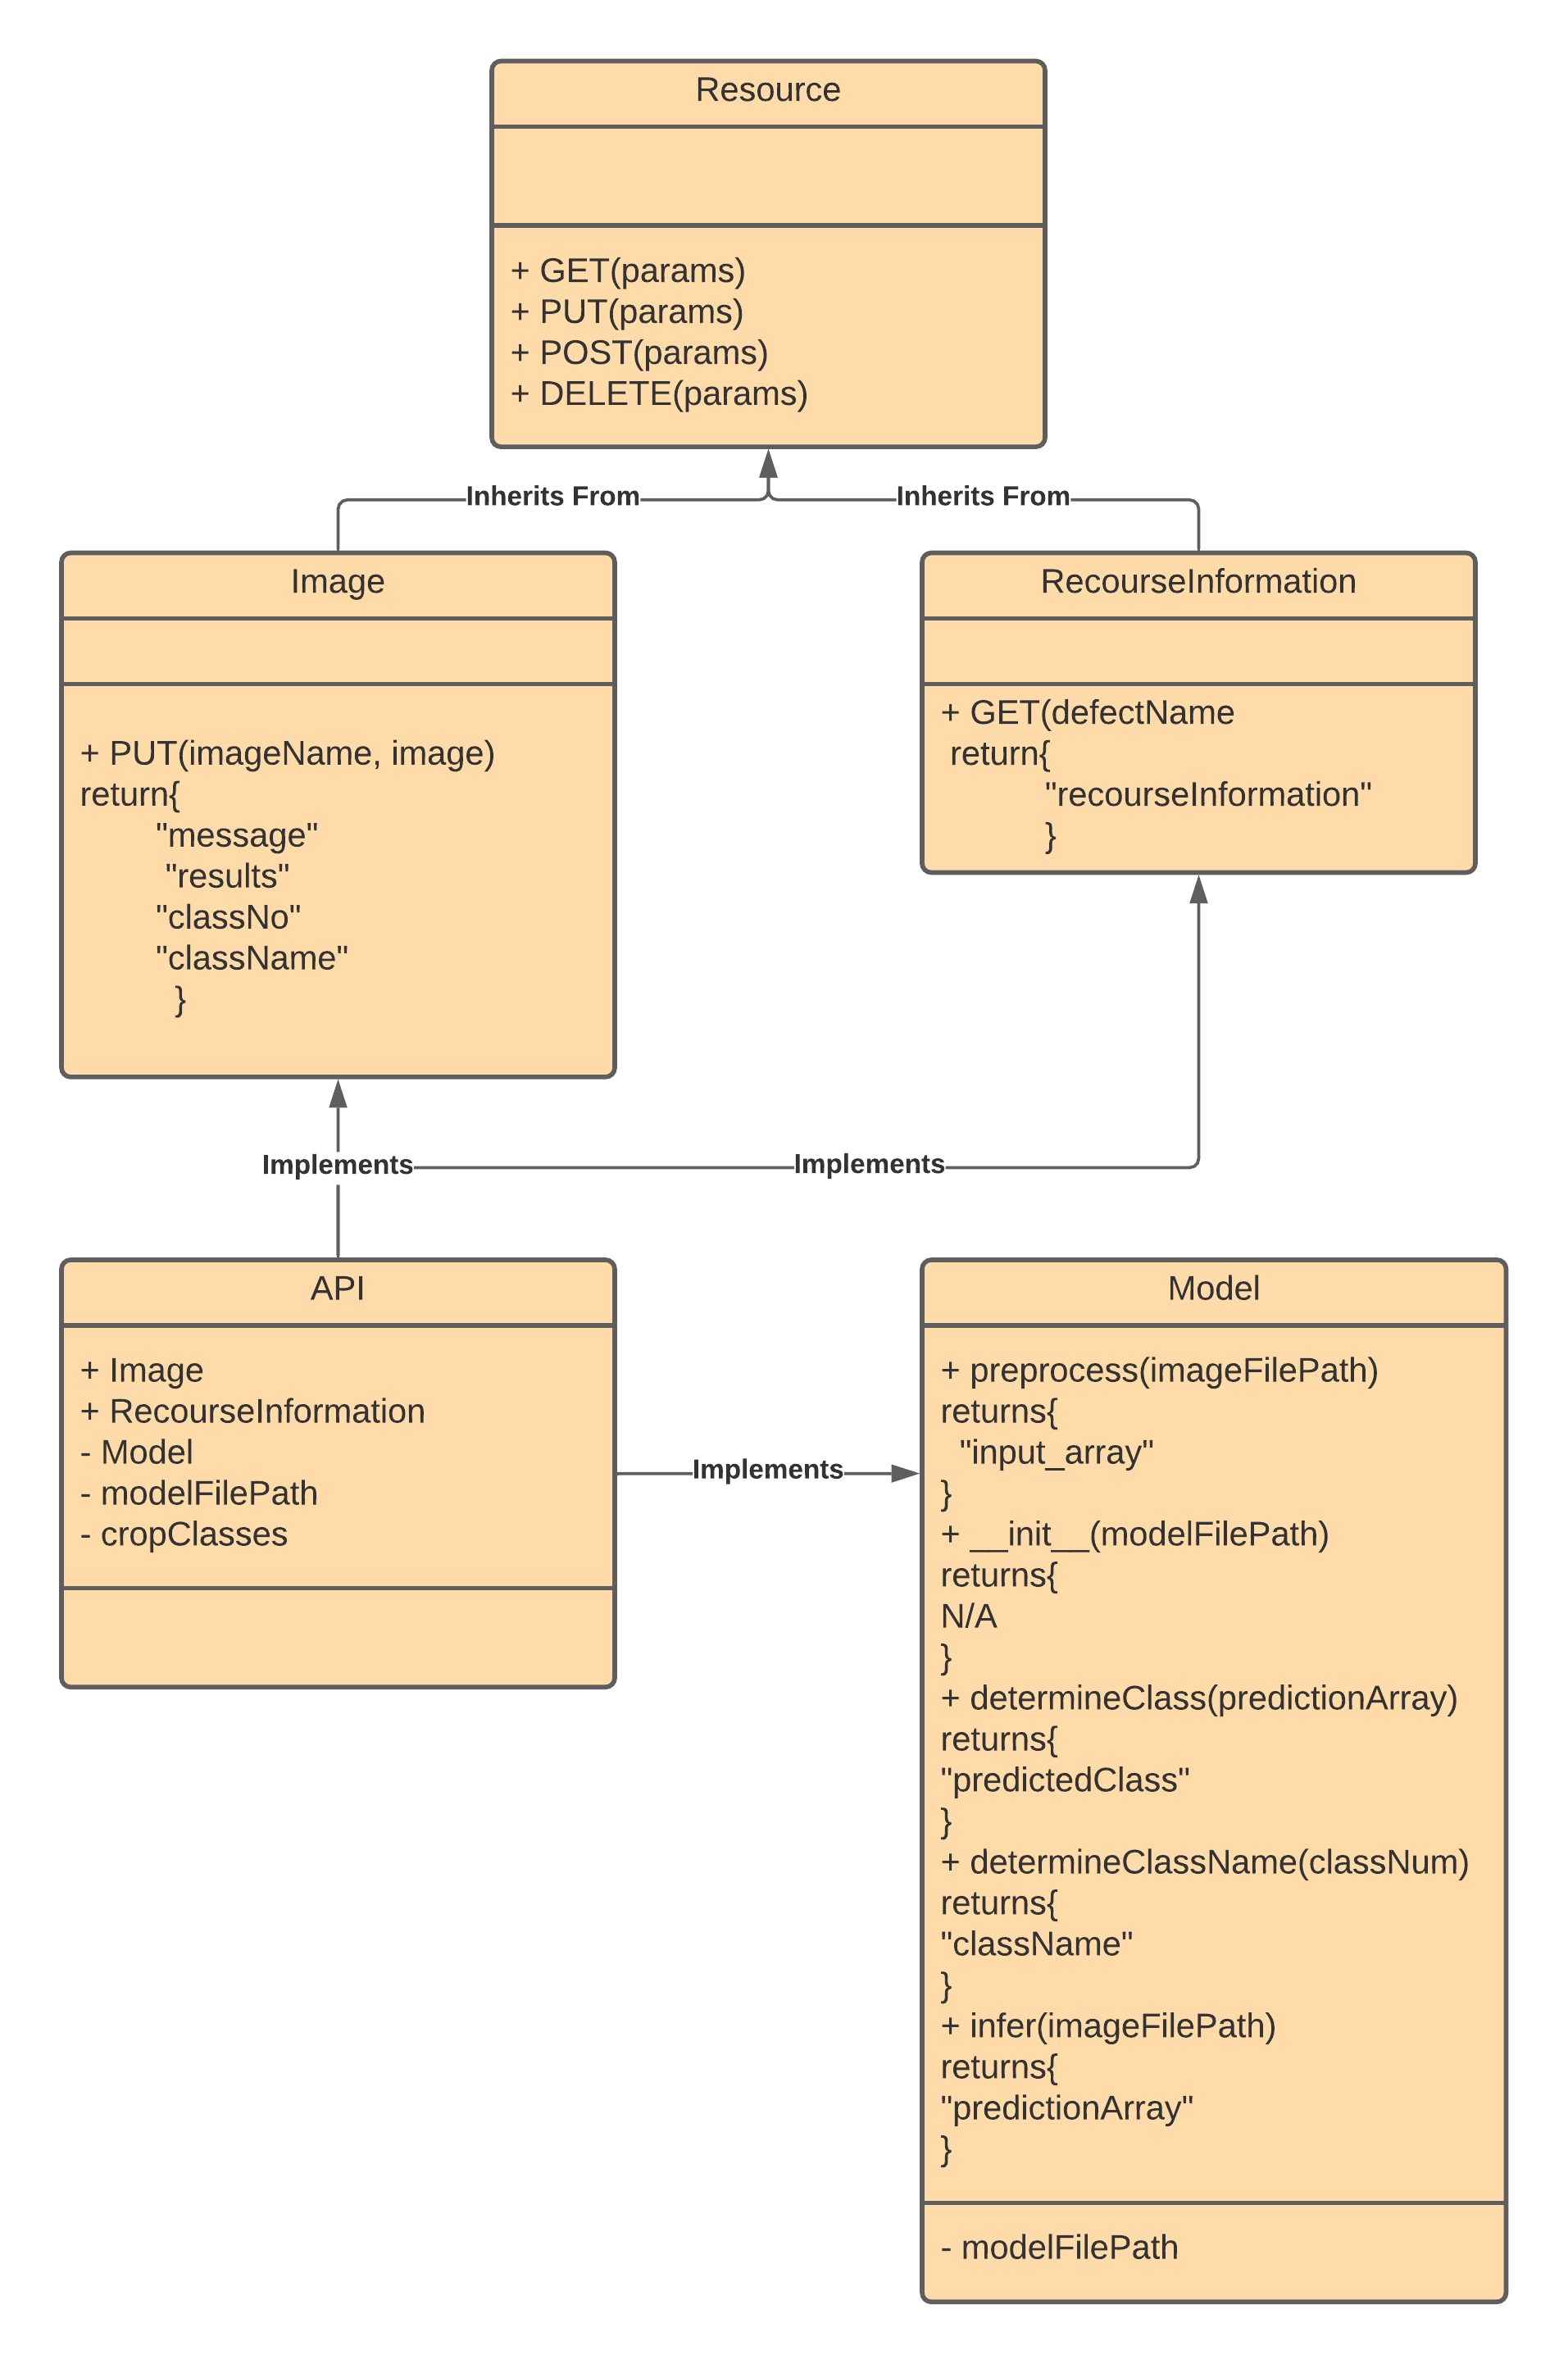
\includegraphics[scale=0.7]{Images/API_InheritenceV3}
        \caption{Backend Class Diagram}
        \label{fig:api_inheritence}
      \end{center}
    \end{figure}

    \subsection{Front-End}
      Using the Vue.js webpack framework means the front-end will be split in to components. A component acting much like an endpoint in an API. Each component will have it's own set of functions and data, with the purpose of seprerating functionality of the UI in to manageable subsets of functionality and styling with the objective being to decouple dependancies between compoonents as much as possible. This helps simplify the development process as it seperates the problem in to distinct parts and it helps with maintinence, allowing them to be tested and developed on in isolation.
      \par
      UI components will be defined using Hypertext Markup language (HTML) and Cascading Style Sheets (CSS). Interativity will be scripted in Javascript. All three extremely common in web development. %With some of the earliest pages of the world wide web in 1990 being defined in HTML1.0 now developed to HTML4.0 (cite html4.0 spec).
      \par
      The main functionality of the web-app will be uploading an image to be analysed by the CNN and recieving a prediciton of which defect is/isn't present. This will be conducted by a single component. Once a prediction has been made, the user can choose to see more information (consisting of images and recourse information) about the defect, which will be handled by a second component.
      \par
      Responses from the API will come in JSON format. With the intention being that as much data processing, such as determining which class is predicted, image preprocessing, and determining of defect image URL's, defect names etc. is handled on the back-end, meaning that any client wishing to interact with the API does not have to implement these features themselves. Therefore all functionality implemented in the web app will concern the consumption of user input and display of API response.

    \subsection{Hosting}
      To make the application accessible on the internet one will utilize virtual machines (VM's) running linux, hosted in the cloud. There will be three VM's, one to host the front-end, one to host the back-end and the other to host the defect images. In all cases nginx will be used to create HTTP servers that will handle all functionality regarding the HTTP protocol and the socket layer.
      \par
      Aside from creating backups of work, version control allows production environments (in this case the VM's) to be easily updated with new features, simply by pulling the latest changes from the repo, installing any new dependencies and re-building the application.


    \subsection{CNN Model Creation \& Integration}
      Seperation of the sofware components allows for the easy interchange of CNN models. This means one can train a model in GoogleColab, utilizing their GPU run-time and save it in the .h5 format. Meaning that, changing the model is as simple as changing a single filepath on the API server. Additionally if one wishes to extend the number of defects (classes) the model is able to predict; a number of steps must take place. Firstly, the filepath to the JSON file defining all classes must be updated on the API to reflect the new set of classes. and the images for the new defect must be added to the image server, or in this case due to hosting limitations, added to the webservice filesystem. Making the process one that is as straightforward as updating two file paths and uploading images using secure file transfer protocol (SFTP) to a server.
      \par
      When training the CNN it isn't clear if 'fine-tuning'(see lit review) an existing CNN is going to be more effective than training a network from scratch. Therefore some experimentation will be nececarry. However, training large networks with millions of parameters can take days or weeks, even when utilizing high end GPU's. For this reason the CNN accuracy is unlikely to acheive state of the art performance in the timeframe available for the project. Fortunately, the application is designed in a way that allows easy swapping of the model when better performance is realised.
      \par
      \subsection{where to put this paragraph?}
      The initial architecture one experimented with was the InceptionNetV3, the rationalle being that one already had a familiarity with the architecture and therefore could rationalise about what may need to change in order to get better performance on the target dataset if initial experiments were not satisfactory. One opted to use a model pre-trained on the ILSSVRC dataset and fine-tune it to suit the crop dataset. This resulted in the model taking around six hours to train over an epoch (using Google Colab GPU runtime) and also drastically overtiffing the training data. One reasoned that the vast number of weights could be to blame for both problems, firstly the more weights the greater the training time, secondly, more filters leads to the network making less generalisations and being able to store many bespoke feature maps to target subsets or perhaps even individual images. Hence when it comes to an unseen example it's feature maps are not generic enough to aid in identifying the unseen image. Therefore one decided to use a a smaller network, 'EfficentNetB0', a network available as a pre-trained\footnote{on the ILSSVRC dataset}[1] CNN through the Keras library. For comparison  the InceptionV3 architecture is 92mb and contains 23,851,784 parameters (weights) whereas the EfficientNetB1 is 29mb and contains 5,330,571 parameters (approx 1/3 the parameters). Fine-tuning this network proved very successfull, acheiving a 98.6\% accuracy. For this dataset, due to the fact all classes the network is classifiying for are relatively similar, less feature maps are needed to generalise about the forms present. To contrast, a network that must classify 100 different classes ranging from a baseball to a shark. with all objects present in different contexts, for instance a closeup of the baseball sat on a table, and a long range shot of it mid flight across the stadium, set against the background of spectators. And it becomes easy to see why so many filters would be nececarry. If we take the crop-example we see all images are closeups of leaves with a neutral background. Therefore it is possible to generalise about this smaller subset of possible images with fewer filters. In fact few parameters becomes a desirable quality of the network as it forces the network to generalise as it does not have the ability to 'memorise' all the individual training images.
      \subsection{where to put this/call this}
      Throughout iterative process of creating the application, the design of the software is affected by factors which have a cause and effect relationship with one another. Such as; designing the system to include a relational database such MySql, as one beleives there may be a need to handle a large amount of  relational data. Later in the project, one realizes they only need the application to be able to retrieve dispirate and simple data, so one drops the database, in favour of using the hierachical storage of the filesystem and structured data languages such as JSON or XML. Another hypothetical example being, one decides to use a novel, bleeding edge, front-end javascript library to aid in creating user-interactive graphing of data. After creating a substantial poriton of the UI functionality, and finding it working smoothly on a high-end desktop PC, one decides to test the application on a smartphone, only to be left with the problem of extremely slow responsiveness. One is then left with the realization, that the novel UI-library is far from optimized and one is now forced in to a bind. If requirments don't specifically request mobile functionality then it would be possible to carry on using the library, however, if one is to take this route, one should have stated in the requirments 'Won't have mobile device support'. However if requirments dictate that mobile support is a 'Must Have' two main possibilites arise, either the library is being used inefectually and time is needed for the developer to become proficcient at using it. Or the library is simply slow. If for whatever reason the library must be dropped from the project, aspects of the UI design will need to change, to better reflect the reduction in expected features; this being caused by the extra time taken to implement what was previously offered by the library. Either this, or extending the project deadline.
      % Such as, adding more libraries to the project will have the knock on effect of increasing the amount of time spent    are one of many factors that feed-into one another such as usability, speed of excecution and speed of creation feed in to one-another.


    \subsubsection{CNN Data and Training}
      One of the most important parts when creating a CNN is the data it is trained on [CITE Halevy]. The more properly labled data the network sees, the better. The most comprehensive dataset available (and the one which will mostly be used) is the Plant Village dataset. it contains 54303 images of healthy and unhealthy leaf images, in 38 catagories divided by species and disease. This dataset also contains pre-segmented\footnote{meaning the background has been blacked out}[1] versions of all the images. This dataset was used in two seperate studies cited in the literature review.
      \par
      Other datasets that may be used to pre-train the network before are the CIFAR10, CIFAR100 \& ILSVRC datasets. These datasets are not specifically plant based, but may benefit the network to build initial feature maps. In \cite{Choi} the authors used networks pre-trained on generic data such as the datasets mentioned. Experiments will be conducted to determine if this benefits classification accuracy

\subsection{Technologies}
  \begin{itemize}
    \item Vue.js
    \begin{itemize}
      \item Vue.js allows for rapid creation of usable websites thanks to its webpack framework, which handles most of the boilerplate needed to handle URL routing and overall structure. It is also considered easy to learn when compared to React and Angular \cite{StudiengangBachelor} which for this project is optimal. Although Vue is currently less popular than React and Angular its popularity is rising, which means its not entirely redundant to learn from an employability standpoint. Vue is a component based framework, meaning it creates a structure to allow the programmer to utilize component technologies to build the website. The component technologies are; custom elements, which allow the programmer to embed javascript code in to either existing HTML elemnts by inheriting from them, or creating entirely new ones. HTML templates, which allows for sections of HTML to be re-used throuought the application, for instance navigation bars. And Shadow DOM's, which allows for DOM elements to contain sub-trees of elements, this is to aid in encapsulating the scope of the contained scripting and styling, meaning individual elements can have their own layers of encapsulation within them.
    \end{itemize}
    \item Bootstrap
        \begin{itemize}
          \item Bootstrap is a CSS framework that has predefined classes for styling HTML elements, this helps with the asthetics of the webpage. For a solo developer this can allow for more time to spent on making the functionality more robust instead of spending time on looks.
        \end{itemize}
    \item Jupyter Notebook / Google Colab
      \begin{itemize}
        \item This pthon environment allows for easy prototyping of code. In the case of Colab, it allows for the usage of google servers and GPUS which can be used to train neural networks. With the benefit of being able to then save the trained weights for usage elsewhere.
      \end{itemize}
    \item Tensorflow \& Keras
      \begin{itemize}
        \item These pthon libraries allow for the creation of complex CNN architectures by abstracting away the underlying matrix/tensor multiplication of deep learning. Allowing for the programmer to declare relationships between CNN features such as convolutional layers, batch normalisation, dropout etc. Without having to construct their inner workings. It also allows for the creation of user defined layers, so adding in ones own bespoke functionality for a layer of the CNN is possible.
      \end{itemize}
    \item NginX
      \begin{itemize}
        \item NginX is a web server. This software, installed on the virtual machines (VM's) hosting, front/back end and files. Handles incoming HTTP protocol requests on ports it is configured to listen to, and serves content accordingly. Additionally, if the need arises, NginX can be used as a load balancer. Taking incoming requests and distributing them amongst the back-end servers via a reverse-proxy. With the reverse-proxy aproach it is also possible to cache response data. Reducing load on the back-end.
      \end{itemize}
    \item Gunicorn
      \begin{itemize}
        \item Gunicorn is another technology used to host the application. This time it is used to interface with the Flask API. It is a Web Server Gateway Interface (WSGI) HTTP server. This gives an interface to the API to allow it to send data back and forth between the web server, NginX.
      \end{itemize}
  \end{itemize}
\section{Requirements}
For assessing requirement priority one will employ the MOSCOW method [CITE Clegg, Dai; Barker, Richard]. This creates subcategory of requirments with the headings Must/Should/Could/Won't - have. The contents of the catagories can change during development in light of development progress. Items placed in the Won't-have category prevent the process of 'scope-creep'.
\begin{itemize}
  \item Must Have
  \begin{itemize}
    \item Ability for user to upload an image
      \begin{itemize}
        \item The user will be able to choose an image file from their local storage using a file explorer popup.
      \end{itemize}
    \item CNN that is capable of classifying at least 2 different defects
      across 2 different plant species.
    \item An API that allows communication from the UI to the CNN
    \item API must be able to receive images.
      \begin{itemize}
        \item Accepted formats being .jpg \& .png
      \end{itemize}
    \item API must return defect information, which will be an array of probability values for each defect class
    \item API must return recourse information.
    \item Application must display images that show the predicted defect.
      \begin{itemize}
        \item These images may be stored either on a seperate server to the front-end. Perhaps in the API servers 'static folder'. Alternatively they will be bundled with the front end.
      \end{itemize}
  	\item The API will be robust enough to handle the receipt of erroneous requests.
  	\item A python backend that will handle image classification using a CNN.
  	\item A UI that will allow the user to upload an image to be analysed.
  	\item The UI will display information regarding the likelihood of each kind of possible defect.
  	\item To display the relevant images that fit the description of the most likely defects.
  	\item To display recourse information to rectify the defect.
  	\item Collecting, cleaning and pre-processing the image data.
    \item Artificially grow the dataset by performing translations/rotations/adding noise to the images to make the training data more comprehensive.
  \end{itemize}
  \item Should Have
  \begin{itemize}
    \item A page to allow users to see a gallery of images sorted by
      defect type.
    \item A page to allow users to see a gallery of images sorted by
      crop type.
    \item The CNN should be able to classify at least 7 different defects across at least two different plant species.
    \item The CNN should acheive at least 80\% accuracy at classifying all different classes of defect in a held out test set that contains an equal number of each class.
  	\item Regularisation techniques to prvent the NN overfitting.
  \end{itemize}
  \item Could Have
  \begin{itemize}
    \item Ability for users to add additional information about the crop
      to determine the defect.
  \end{itemize}
  \item Won't Have
\end{itemize}
\section{Testing and Implementation details}


\section{Justification of Implementation Choices}
